\subsection{Dati e risultati}

\paragraph{Comparatore.}

Lo scopo della realizzazione di qusto circuito è famigliarizzare con il comparatore LM311. Il primo circuito che abbiamo montato, in figura
\ref{fig:comparatore4}, è il più semplice utilizzo di questo componente. L'ingresso è
impostato sul piedino non invertente in modo da ottenere un comparatore non invertente.
L'ingresso invertente è invece collegato a comune e definisce la soglia di riferimento per
la comparazione (mettendolo a comune la soglia è quindi 0 V). Collegando questo ingresso
ad una tensione continua a scelta, il comparatore comparerà il segnale in ingresso alla
tensione scelta.

\begin{SCfigure*}
	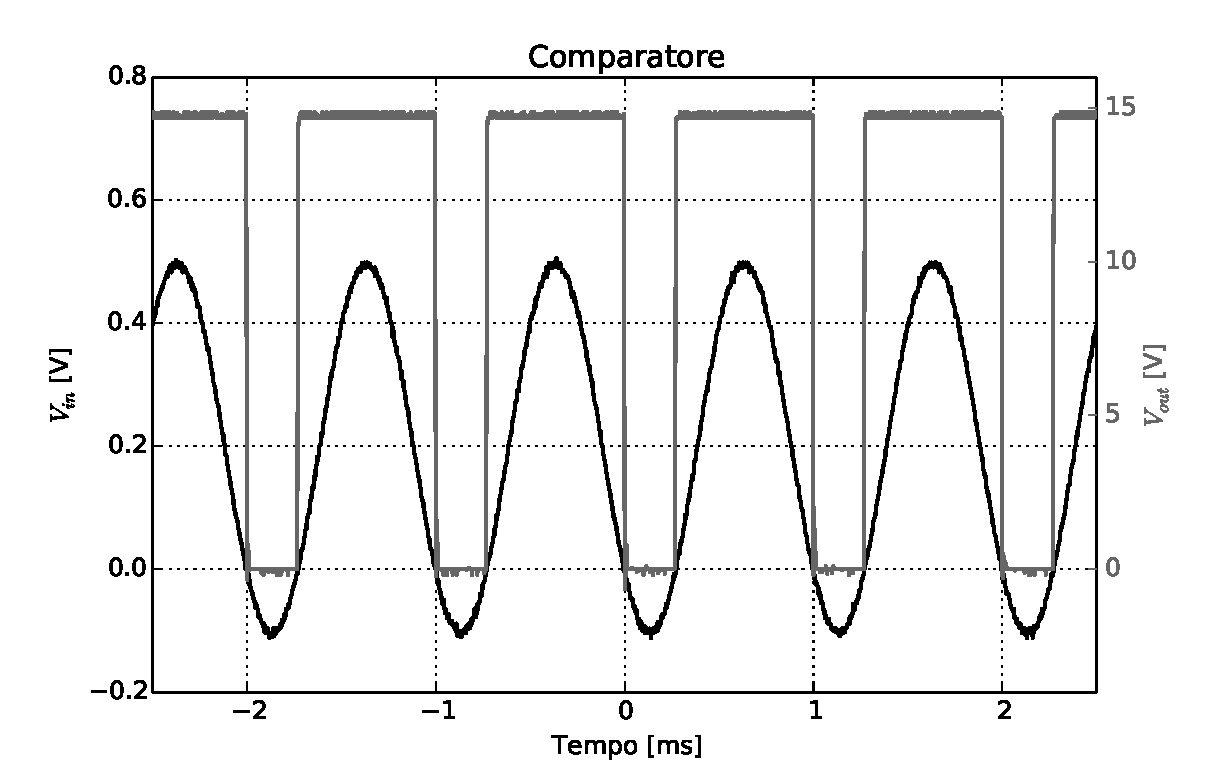
\includegraphics[width=0.75\textwidth]{figure/comp_graph.pdf}
	\caption{Esempio di funzionamento del circuito \ref{fig:comparatore4}. Il segnale in ingresso
		è la sinusoide di 600 mVpp a 1 kHz con un offset di +200 mV (la scala per l'ingresso è a 
		sinistra, per l'uscita è a destra). Come si può notare il circuito
		compara correttamente il segnale in ingresso con il comune, fornendo una specie di onda quadra
		all'uscita. Gli effetti del rumore non sono visibile a questa scala di tempo, ma sono visibili in
		figura \ref{fig:rumore4}.}
	\label{fig:comp_graph4}
\end{SCfigure*}

Il comparatore LM311 funziona in modo un po' diverso dall'UA741. Essenzialmente agisce come
se al suo interno ci fosse un interruttore con i capi collegati all'uscita e a comune
(l'LM311 ha un piedino da collegare a ground, mentre per l'UA741 non era necessario).
L'interruttore è interdetto se $V^+ > V^-$ ed è chiuso in caso contrario.
Quindi quando l'ingresso non invertente $V^+$ è ad una tensione maggiore di quello invertente $V^-$
l'uscita è a + 15 V (alimentazione) a causa della resistenza di pull-up R.
Invece, se $V^- > V^+$, l'uscita è a comune. La resistenza R è stata scelta
''grande`` (\SI{10}{\kilo\ohm}) per evitare il passaggio di troppa corrente e la conseguente
dissipazione di potenza nel caso di uscita a ground.
Per le altre specifiche del circuito si faccia riferimento alla figura \ref{fig:comparatore4}.

Quindi abbiamo un circuito che confronta un segnale con lo zero e fornisce in uscita uno stato binario:
$V\ped{sat}^+$ se il segnale è maggiore di zero e 0 V se il segnale è minore di zero.
Per testarne il funzionamento abbiamo fornito in ingresso vari segnali con il generatore di funzioni
d'onda. Un esempio è riportato in figura \ref{fig:comp_graph4}.

Il problema principale di questo circuito è il fatto che è soggetto al rumore. Nelle vicinanze di
una transizione da positivo a negativo possono esserci più punti che intersecano il riferimento a causa
del fatto che c'è sempre rumore sommato al segnale. Noi lo abbiamo
testato con funzioni d'onda di ampiezza picco-picco piuttosto ridotta (200 mV e 600 mV) per
far si che la transizione fosse più lenta e gli effetti del rumore risultassero più evidenti.
Il rumore è visibile in figura \ref{fig:rumore4}.

\paragraph{Trigger di Schmitt.}

Per evitare questo problema del rumore si utilizza il cosiddetto trigger di Schmitt, ovvero un circuito
come quello riportato in figura \ref{fig:trigger_schmitt4}. Il trigger di Schmitt è un comparatore con isteresi,
vale a dire un comparatore che invece di scattare al passaggio di una soglia, ha una fascia di tensioni
in cui non agisce e scatta solo quando il segnale esce da questa banda. La figura \ref{fig:comp_ist_exp4} chiarifica
il funzionamento.

\begin{figure}[t]
    \centering
    \small
    \def\svgwidth{\columnwidth}
    \subimport{figure/}{ist.pdf_tex}
	\caption{Funzionamento di un comparatore con isteresi. Il passaggio tra i due stati
        di uscita del comparatore avviene non ad una determinata soglia, ma all'uscita della
        banda di tensioni compresa tra due soglie $V\ped{OH}$ e $V\ped{OL}$. In questo modo il
        comparatore è molto meno soggetto al rumore.}
	\label{fig:comp_ist_exp4}
\end{figure}

Ma come è possibile ottenere un effetto simile in un circuito? La soluzione è utilizzare un feedback \emph{positivo}
come indicato in figura \ref{fig:trigger_schmitt4}. In questa configurazione (è evidentemente possibile costruire un trigger
simile in configurazioni diverse), le resistenze $R_1$ ed $R_2$ formano un partitore che determina
la tensione $V^+$ all'ingresso non invertente, determinando così la grandezza della banda dove il comparatore non agisce.

Se la tensione $V\ped{in}$ supera lo zero, anche la tensione $V^+$ lo supera, ed il comparatore interdetto costringe
$V\ped{out}$ a rimanere alla tensione alta (che in questo caso varia con la tensione in ingresso. Se le tensioni in ingresso
sono piccole rispetto a 15 V, si ottiene un uscita di (15 V)$\cdot(R_1 + R_2)/(R_1 + R_2 + R_3) = 13.6$ V). In seguito, quando $V\ped{in}$ scende
sotto lo zero, il partitore fa si che la tensione in $V^+$ sia ancora maggiore di zero, evitando così la commutazione del comparatore.
Ovviamente ad un certo punto, quando $V\ped{in}$ supera la tensione di soglia negativa $V\ped{OL}$ (determinata dalle resistenze)
anche $V^+$ diventa minore di zero e $V\ped{out}$ viene messo a terra. Da questo punto in poi il partitore funziona in modo
diverso, infatti $R_3$ non ne fa più parte. Quindi quando la tensione sale nuovamente, si ha che il segnale in ingresso deve
superare lo zero (la soglia alta $V\ped{OH}$) affinché $V^+$ superi lo zero facendo chiudere il comparatore e riportando tutto alle condizioni iniziali.
Si ha quindi un comportamento di isteresi, con tensioni in salita trattate in maniera differente da quelle in discesa.
Il punto principale del discorso è che se l'ampiezza tipica del rumore è minore dell'ampiezza della banda, il comparatore
sarà molto meno soggetto a scatti casuali.

Per il circuito abbiamo scelto $R_1 = \SI{100}{\ohm}$, $R_2 = \SI{100}{\kilo\ohm}$ e $R_3 = \SI{10}{\kilo\ohm}$.
In questo modo, valendo la formula

\begin{equation}
    V^+ = V\ped{in} + (15\;\text{V} - V\ped{in}) \frac{R_1}{R_1+R_2+R_3}
\end{equation}

si ottiene che

\begin{equation}
    V\ped{in} = V^+ \frac{R_1+R_2+R_3}{R_2+R_3} - 15 V \frac{R_1}{R_2+R_3}
\end{equation}

Imponendo $V^+ = 0$ ed inserendo i valori da noi scelti, risulta

\begin{equation}
    V\ped{OL} = - 15 V \frac{R_1}{R_2+R_3} = -\SI{13.6}{\milli\volt}
\end{equation}

Poiché $V\ped{OH} = 0$, la fascia di tensioni ``di isteresi'' è ampia 13.6 mV, 
che è dell'ordine del rumore presente nel nostro circuito. La figura \ref{fig:rumore4} mostra gli effetti dell'isteresi
sul rumore. In figura è visibile il circuito del paragrafo precedente e quello con isteresi, che presenta molto meno rumore.
Aumentando $R_1$ è possibile aumentare la banda ``di isteresi'' e quindi diminuire ancora il rumore (l'ovvio svantaggio è che
si perde sensibilità nella comparazione, quindi è sconveniente aumentare troppo le soglie).
Notare che sarebbe stato possibile avere una banda simmetrica rispetto allo zero, mettendo $V^- = -\SI{13.6}{\milli\volt}/2$
anche se questo può portare a rumore ulteriore.

\begin{SCfigure*}[1][t]
    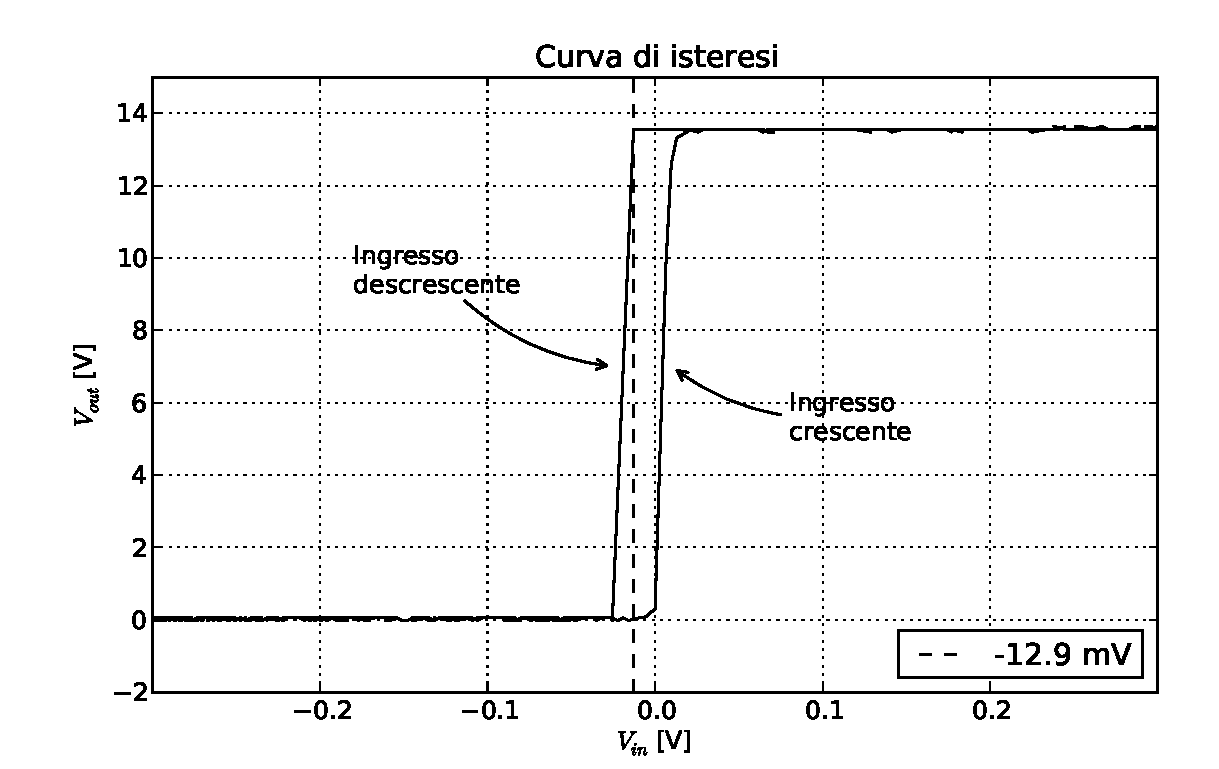
\includegraphics[width=0.75\textwidth]{figure/isteresi.pdf}
    \caption{Curva di isteresi del trigger di Schmitt. La curva di isteresi si ottiene graficando la tensione in output versus la tensione
        di input. In questo caso l'input va da - 0.3 V a 0.3 V e ritorno. Si vedono bene le due soglie e la banda di
        isteresi. L'ampiezza dell'output è 13.7 V.}
	\label{fig:isteresi4}
\end{SCfigure*}

Con l'oscilloscopio abbiamo misurato la tensione $V\ped{OL}$, rilevando $14.1 \pm 0.1$ mV, vicino al valore calcolato.
La discrepanza è spiegabile grazie al fatto che era presente rumore dell'ordine di grandezza della soglia e quindi
è difficile capire dove veramente inizia la commutazione.

Abbiamo inoltre acquisito i dati e graficato la curva di isteresi del circuito. Il risultato è visibile in figura \ref{fig:isteresi4}.
Si vedono bene le due soglie $V\ped{OL}$ e $V\ped{OH}$, anche se nell'intervallo dove il comparatore commuta ci sono pochi
punti, che in parte spiegano il fatto che le soglie siano oblique. Con questo metodo $V\ped{OL} = 12.9$ mV, mentre $V\ped{OH}$ è
vicina a 0 V.

\paragraph{Oscillatore a rilassamento.}

Passiamo ora all'analisi di un circuito completamente diverso, l'oscillatore a rilassamento riportato in
figura \ref{fig:oscillatore4}. Questo circuito genera un onda quadra di ampiezza $V\ped{sat}^+ - V\ped{sat}^-$
e di frequenza regolabile da 370 Hz a 438 Hz tramite il trimmer sulla retroazione negativa. Si noti che in questo
circuito abbiamo usato l'UA741.

Come funziona questo circuito? All'accensione del circuito l'uscita si trova, per esempio, a $V\ped{sat}^+$ (a causa
della tensione di offset o di altri disturbi, come abbiamo visto nella precedente relazione). Questo significa che
$V\ped{B} = V\ped{sat}^+/2$ e che, grazie alla retroazione negativa, il capacitore inizi a caricarsi.
L'uscita resta a $V\ped{sat}^+$ finché ai capi del condensatore la tensione non supera $V\ped{B} = V\ped{sat}^+/2$, dopodiché
l'operazionale porta l'uscita a $V\ped{sat}^-$. In seguito $V\ped{B} = V\ped{sat}^-/2$ e il condensatore si scarica
e carica con polarizzazione inversa, fino a che ai sui capi non c'è una tensione pari a $V\ped{B} = V\ped{sat}^-/2$. Al che
l'operazionale porta l'uscita a $V\ped{sat}^+$ ed il ciclo ricomincia. La frequenza del ciclo è determinata dalla resistenza
sulla retroazione negativa, che limita la corrente di carica del condensatore e quindi la velocità di carica.
A resistenze più basse corrispondono frequenze più alte e viceversa.

Dopo aver montato il circuito ne abbiamo verificato il funzionamento, che è risultato corretto. L'ampiezza picco-picco dell'onda quadra generata
è stata misurata ed era pari a 27.3 V, indipendentemente dalla frequenza generata. Quindi $V\ped{sat}^{\pm} = \pm 13.7$ V.

Usando la definizione di capacità, la legge di Ohm e risolvendo l'equazione differenziale nel caso in cui $V\ped{out} = V\ped{sat}^+$,
si ottiene l'equazione che descrive la carica del condensatore. Imponendo come condizioni inziali che a t = 0 si avesse $V\ped{A} = V\ped{sat}^-/2 = -V\ped{sat}^+/2$
(ovvro che l'uscita abbia appena commutato verso $V\ped{out} = V\ped{sat}^+$),
e risolvendo per t si ottiene

\begin{equation}
    t = \frac{T}{2} = RC\log\left(\frac{2}{3} - \frac{2}{3}\frac{V\ped{A}}{V\ped{sat}}\right)
\end{equation}

Per calcolare il periodo dell'onda possiamo quindi porre $V\ped{A} = V\ped{sat}^+/2$. Facendo l'inverso del periodo si ottiene la frequenza:

\begin{eqnarray}
    f\ped{R_v = 0} = 460 \pm 90 \; \si{\hertz} \\ f\ped{R_v = \SI{10}{\kilo\ohm}} = 230 \pm 50 \; \si{\hertz}
\end{eqnarray}

Per il calcolo delle incertezze, abbiamo assunto un incertezza del 5\% sulle resistenze e del 20\% sulla capacità,
ovvero le tolleranze dei componenti usati. Le misure hanno rivelato valori $f\ped{R_v = 0} = 438 \; \si{\hertz}$
e $f\ped{R_v = \SI{10}{\kilo\ohm}} = 298 \; \si{\hertz}$, il primo dei quali è compatibile con i nostri risultati, mentre il secondo no
(non sappiamo perché).

\paragraph{Interruttore crepuscolare.}

\begin{figure*}
    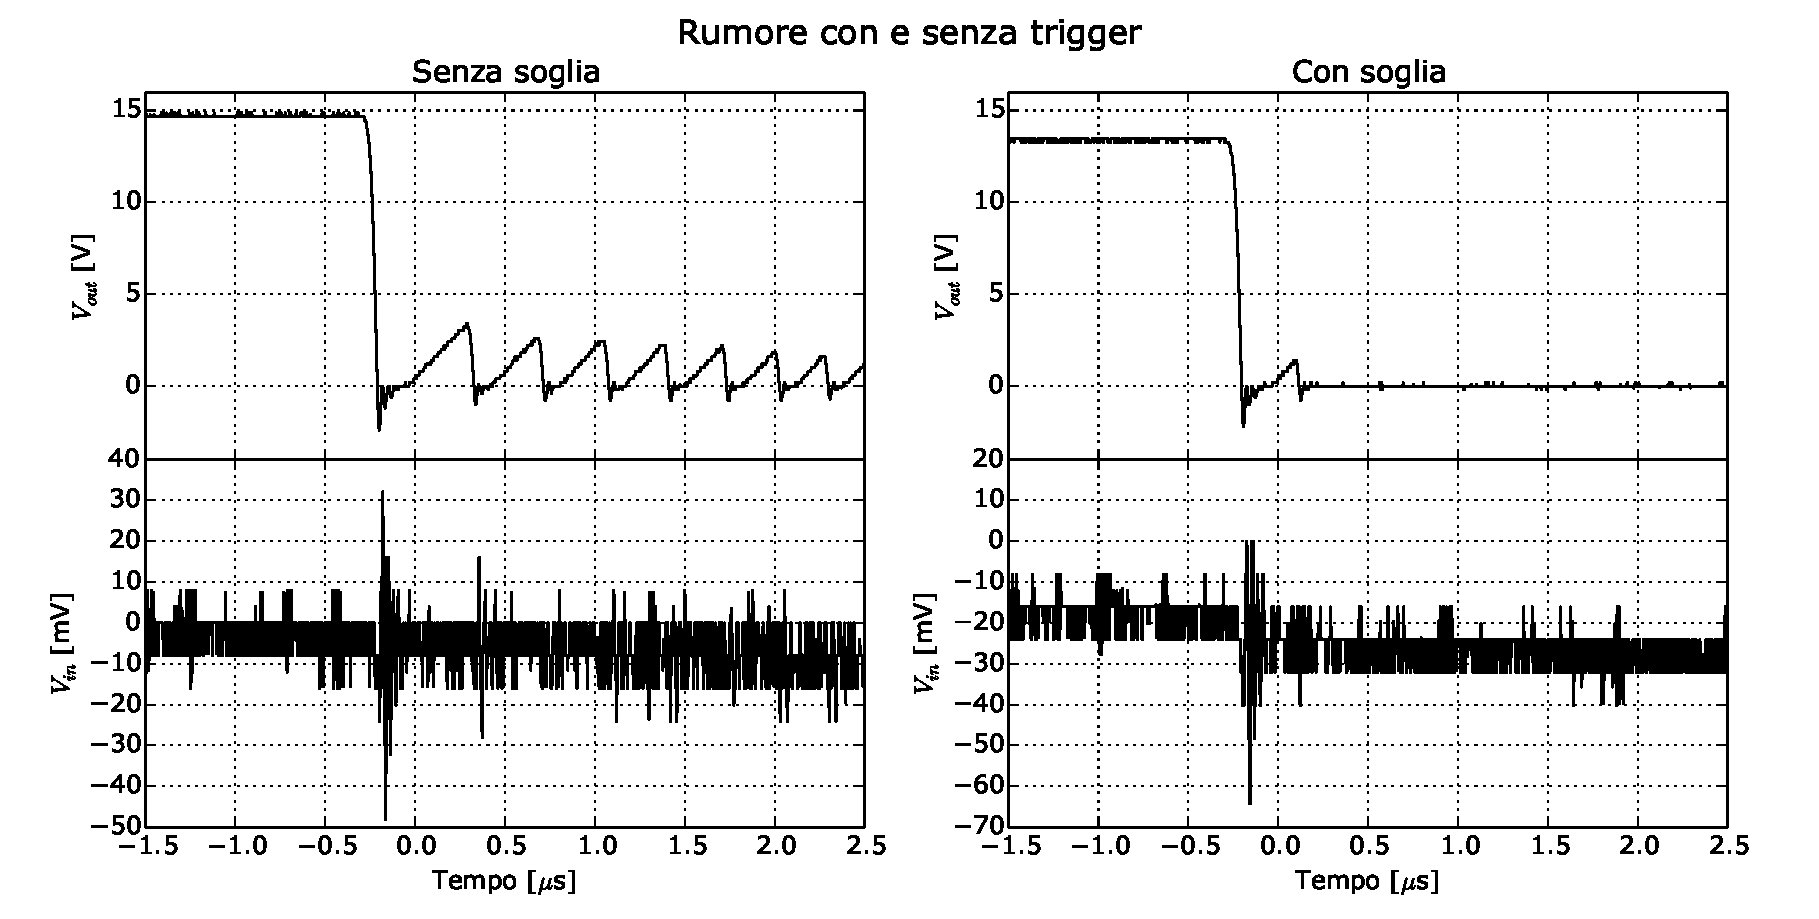
\includegraphics[width=\textwidth]{figure/trigger_graph.pdf}
    \caption{Nel grafico a sinistra è riportato l'output del circuito \ref{fig:comparatore4} (in alto) e l'ingresso dello stesso circuito,
        riportato in scala molto ingrandita per visualizzare il rumore. Stessa cosa per la figura a destra, solo che in questo caso
        il circuito è il trigger di Schmitt (\ref{fig:trigger_schmitt4}). Evidentemente il rumore è molto minore. Si notino le scale temporali
        (per questo il rumore non è visibile nella figura \ref{fig:comp_graph4}) e l'ampiezza del rumore in uscita (vari Volt). Nell'immagine a destra
    si nota inoltre che la commutazione avviene circa ai -13.6 mV previsti.}
	\label{fig:rumore4}
\end{figure*}

L'ultimo circuito che abbiamo realizzato è una semplice ma molto interessante applicazione del trigger di Schmitt.
Si tratta di un circuito che analizza il segnale proveniente da un fototransistor
(un transistor simile ad un BJT ma controllato dalla luminosità ambientale invece che dalla corrente di base)
e che accende o spegne un LED in base a tale segnale. Una versione modificata del circuito può essere utile
per accendere delle luci automaticamente la sera o in altre situazioni simili. Il diagramma schematico del
circuito è mostrato in figura \ref{fig:crepuscolare4}.

Nel circuito, la corrente che attraversa il fototransistor Q dipende dalla luminosità dell'ambiente attorno al transistor.
Il transistor è collegato a - 50 mV invece che a comune per assicurare una corretta polarizzazione del trasistor in qualsiasi
condizione operativa. L'amplificatore UA741 serve, assieme alla retroazione $R_1$, ad amplificare la corrente forrnita dal
fototransistor e a convertirla in tensione. Abbiamo verificato che la corrente massima che il transistor assorbe (in condizioni di
massima luminosità) è di circa 14 $\mu$A; consequentemente è stata usata una resistenza $R_1 = 1$ \si{\mega\ohm} per trasformare
la corrente di un segnale di qualche Volt.
Nello stadio successivo, troviamo il comparatore LM311 all'interno di un trigger di Schmitt, che compara il segnale amplificato
con una soglia regolabile tramite la resistenza variabile $R_v$. Nel feedback positivo troviamo due resistenze $R_2 = 10$ \si{\kilo\ohm}
ed $R_3 = 100$ \si{\kilo\ohm} che fanno si che le soglie $V\ped{OL}$ e $V\ped{OH}$ siano piuttosto distanti e che il circuito
sia poco soggetto al rumore (vogliamo che il LED si accenda e si spenga in modo stabile; vorremmo evitare di vedere il LED
accendersi e spegersi ripetutamente a causa di variazioni di luminosità repentine). In seguito abbiamo un ramo che collega l'uscità
dell'LM311 con l'alimentazione positiva mediante una resistenza (limitatore di corrente) e il diodo LED.

Quando la luce ambientale è alta, il fototransistor assorbe molta corrente, e all'ingresso non invertente dell'LM311 arriva una
tensione alta. Se la tensione supera la soglia impostata dall'utilizzatore, il comparatore è in interdizione e attraverso il diodo
passa pochissima corrente, non sufficiente ad illuminarlo. Quando l'ambiente è poco luminoso il transistor assorbe poca corrente,
all'ingresso del comparatore arriva una tensione bassa e il comparatore mette a terra la sua uscita. Quindi scorre una corrente
$I = \frac{15 V}{R_4} = 15$ mA attraverso il diodo. Questa corrente è sufficiente per far funzionare il LED.

Dopo aver montato il circuito (tra molte peripezie a dire il vero), abbiamo verificato il suo funzionamento, che è risultato
estremamente stabile. Il diodo si illumina nel momento in cui è utile che lo faccia (quando la luminosità diventa scarsa)
ed è totalmente assente qualsiasi scatto del LED dovuto a rumore (ricordiamo che le stesse lampade del laboratorio si accendono
e si spengono alla frequenza della rete, ovvero 50 Hz).
